% A control jump changes the derivative while the state remains continuous.
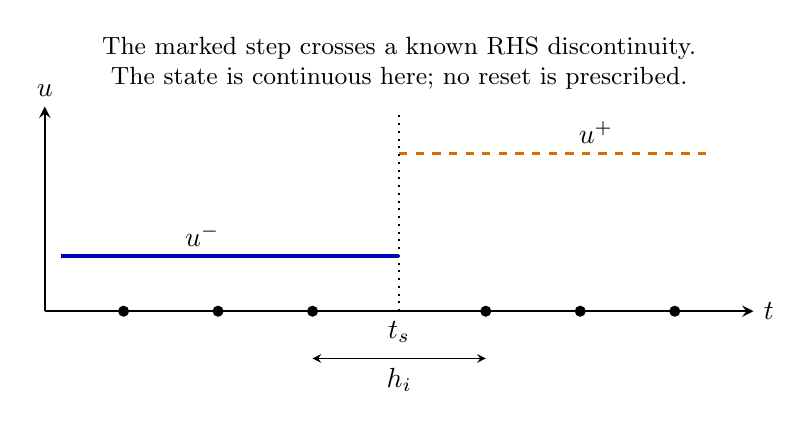
\begin{tikzpicture}[>=stealth,font=\normalsize]
\draw[->,thick](0,0)--(9,0)node[right]{$t$};\draw[->,thick](0,0)--(0,2.6)node[above]{$u$};
\draw[blue!70!black,very thick](.2,.7)--(4.5,.7);
\draw[orange!85!black,very thick,dashed](4.5,2)--(8.5,2);
\draw[dotted,thick](4.5,0)--(4.5,2.5);\node[below]at(4.5,0){$t_s$};
\node[above]at(2,.7){$u^-$};\node[above]at(7,2){$u^+$};
\foreach \x in {1,2.2,3.4,5.6,6.8,8}{\fill(\x,0)circle(2pt);}
\draw[<->](3.4,-.6)--node[below]{$h_i$}(5.6,-.6);
\node[font=\small,align=center]at(4.5,3.15){The marked step crosses a known RHS discontinuity.\\The state is continuous here; no reset is prescribed.};
\end{tikzpicture}
